\section{Introduction: Definitions and Preliminaries}

\begin{definition}\label{def:simplicial-complex}
    A \define{simplicial complex} is a hypergraph \(G = (V,E)\) that is closed under \textit{downward containment} i.e 
    \begin{equation}
        S \in E, S^{\prime} \subset S \implies S^{\prime} \in E 
    \end{equation} 
    Every \(S \in E\) is called a \define{face}
\end{definition}

We usually partition the faces of our simplicial complex according to their sizes. 

\begin{definition}
    Given a simplicial complex \(X\)
    \begin{equation}
        X = X(0) \cup X(1) \cup X(2) \dots \cup X(d)
    \end{equation} 
    where \(X(i)\) denotes the faces of size \(i+1\) - and is said to have a \define{dimension} \(i\).    
\end{definition}

The notion of link is a rather important concept. 

\begin{definition}
    Given \(X\) a \(d\)- dimensional complex and \(s \in X(i)\), the \define{link} of \(s\) is 
    defined as follows: 
    \begin{equation}
        X_s \triangleq \{ t \in X \mid s \cup t \in X, s \cap t = \emptyset \} 
    \end{equation}   
\end{definition}

It can be thought of as a generalization of the concept of the neighborhood of a graph, but for simplicial complexes. 

\begin{definition}
    Given \(X\), a simplicial complex and \(k < d\), for some non-negative \(k\). The \define{\(k\)-skeleton} of \(X\) 
    is the subspace of \(X\) that is the union of faces of dimension \(\leqslant k\).  
\end{definition}

\begin{definition}
    We say that a complex is a \define{pure \(d\)-dimensional} is every 
    maximal face is of dimension exactly \(d\). 
\end{definition}

Using these objects, we are ready to define the notion of expansion over 
simplicial complexes. 

\begin{definition}
    We say that \(X\), a pure \(d\)-dimensional simplicial complex, is a 
    \define{\(\lambda\)-one-sided HDX} (resp. \(\lambda\)-two-sided HDX) if 
    \begin{itemize}
        \item \(1\)-skeleton of \(X\) is a \(\lambda\)-one-sided expander (resp. \(\lambda\)-two-sided expander)  
        \item \(\forall i \leqslant d-2, \  s \in X(i)\), the 1-skeleton of \(X_s\) is a \(\lambda\)-one-sided expander 
        (\(\lambda\)-two-sided expander)    
    \end{itemize}
\end{definition}

\begin{definition}
    A \define{weighted pure simplicial complex} is a pair \((X, \Pi)\) where \(X\) is 
    a pure \(d\)-dimensional simplicial complex endowed with a distribution \(\Pi 
    = \left(\pi_{0}, \pi_1, \dots , \pi_d \right)\) over 
    each level such that:     
    \begin{itemize}
        \item \(\pi_i\) is a distribution over \(X(i)\) for all \(i = 0, 1, \dots , d\)  
        \item \(\pi_d\) is arbitrary
        \item For all \(0 \leq i \leq d\) and \(\tau \in X(i)\), \(\pi_i(\tau)\) is the 
        probability that \(\tau\) is selected via the following process: 
        \begin{enumerate}
            \item Draw a \(d\)-face \(\sigma\) from \(\pi_d\) 
            \item Pick an \(i\)-face \(\tau \subset \sigma\) where \(\abs{\tau} = i \)  
        \end{enumerate}     
        Equivalently, 
        \begin{equation}
            \pi_i (\tau) = \frac{1}{\binom{d}{i}} \sum_{\substack{\sigma \in X(d)\\ \tau \subset \sigma}} \pi_d(\sigma) 
        \end{equation}
    \end{itemize}
\end{definition}

For any \(0 \leq i < d\), \(\pi_i\) can be thought of as distribution induced by \(\pi_d\). The \define{weighted links} of a weighted complex are themselves weighted complexes with distribution inherited from the global distribution.

\begin{definition}
    Let \((X, \Pi)\) be a \(d\)-dimensional weighted simplicial complex. For all \(0 \leq i \leq d\) and \(\tau \in X(i)\), the weighted link \((X_\tau, \pi_\tau)\) is defined as follows:
    \begin{itemize}
        \item \(X_\tau =  \{ \sigma \mid \sigma \cup \tau \in X, \sigma \cap \tau = \emptyset \}  \) 
        \item \(\pi_{\tau, d - i}(\sigma) = \frac{\pi_{d}(\sigma \cup \tau)}{\sum_{\psi\in X_{\tau}(d - i)} \pi_{d}(\psi \cup \tau)}\)
    \end{itemize}
\end{definition}

There is a notion of expansion of expansion over this general object, i.e. a weighted simplicial
complex. 

\begin{definition}[Weighted Spectral Expander]
    A weighted simplicial complex \((X, \Pi)\) is a (one-sided/two-sided) \define{\(\lambda\)-local spectral expander} if the underlying graph of every weighted \(i\)-link, for \(0 \leq i \leq d-2\) is a (one-sided/two-sided) \(\lambda\)-spectral expander.
\end{definition}



\begin{figure}
    \centering 
    \begin{subfigure}{.5\textwidth}
        \centering
        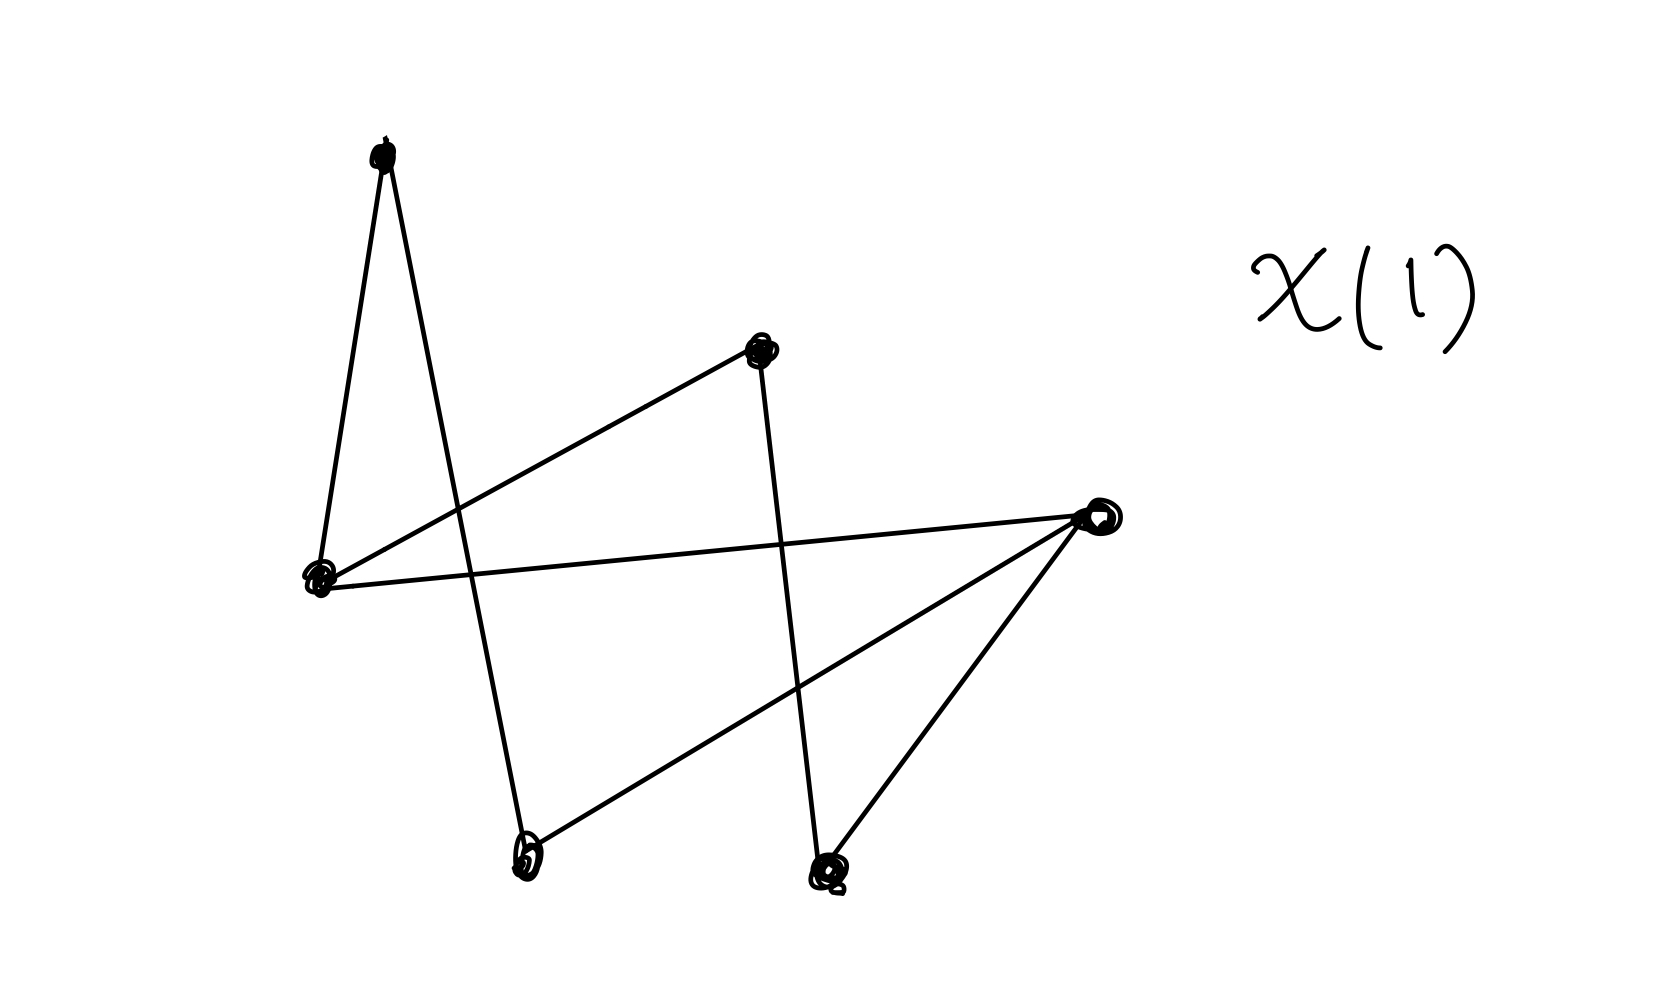
\includegraphics[scale=.1]{fig/dim-1.jpeg}
        \caption{1-skeleton of a complex}
    \end{subfigure}%
    \begin{subfigure}{.5\textwidth}
        \centering
        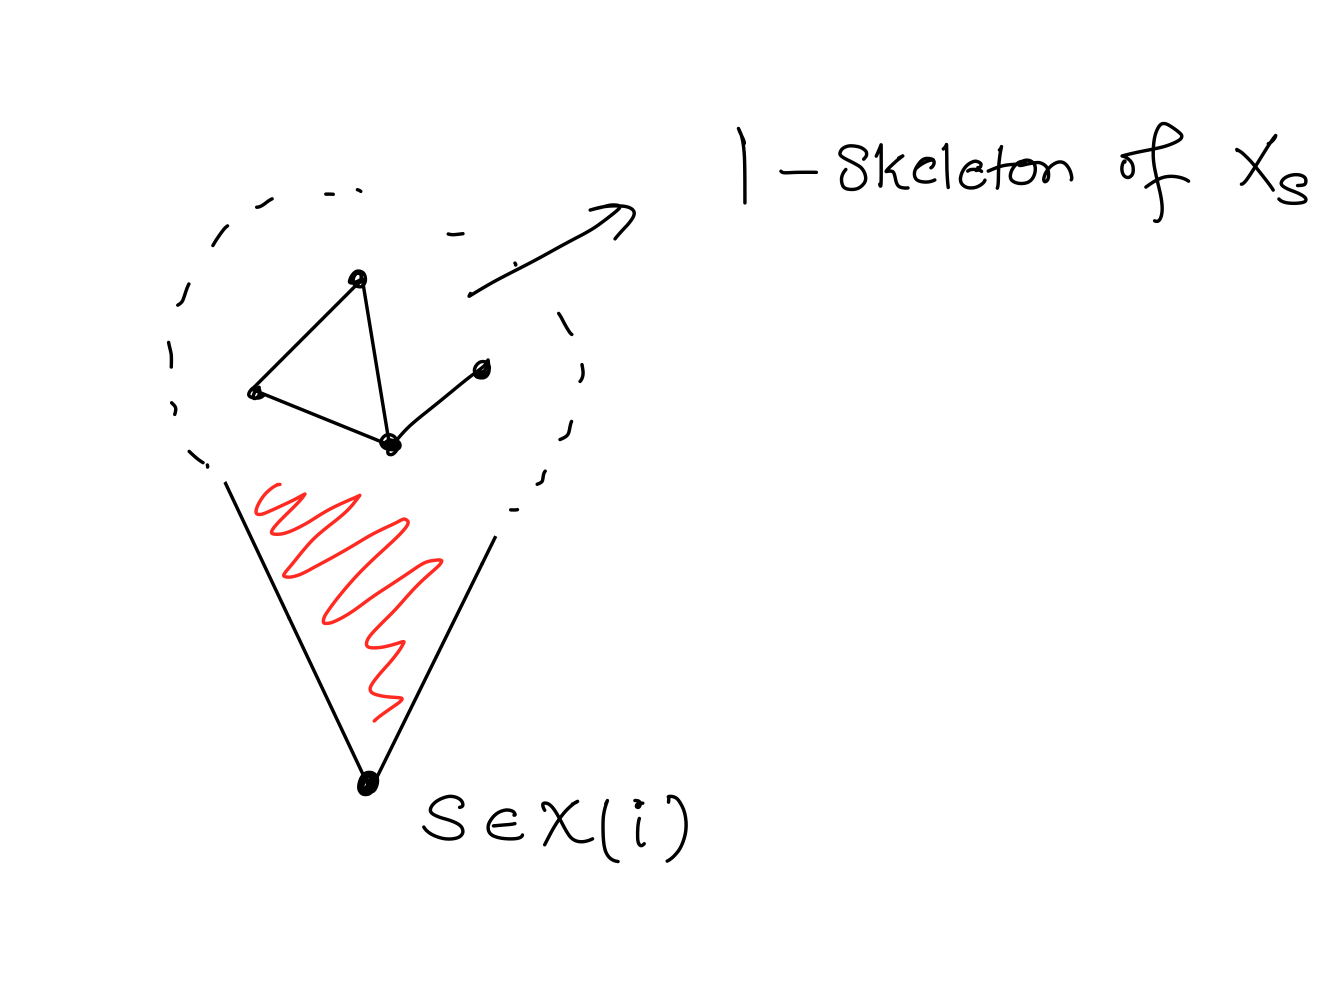
\includegraphics[scale=.15]{fig/1-skel.jpeg}
        \caption{1-skeleton of link corresponding to \(s\)}
    \end{subfigure}
\end{figure}

A central theme of these notes is to understand how we might construct two-sided HDXs with bounded degree. 

\begin{definition}
    We say that \(X\) is 
    \define{\((r_0, r_1 \dots r_{d-1})\)-regular} if for \(0\leqslant i \leqslant d-1\)
    every \(s \in X(i)\) is contained in \(r_i\) \((i+1)\)-faces.        
\end{definition}

As it turns out, many important examples of HDXs are, in fact, not regular. However, assuming 
helps us avoid messy calculations, at least for now. Before we proceed, we discuss a few example 

\begin{example}[\(d\)-dimensional complete complex]
    The \(n\)-simplex, denoted as \(\Delta^n\) is the \(n\)-dimensional simplicial 
    complex that contains all subsets of \(n+1\) elements. The \(d\)-dimensional 
    complete complex on \(n\) vertices is the \(d\)-skeleton of \(\Delta^{n-1}\).
    Namely, these are all the subsets \([n]\) with size \(d+1\). The 
    \(1\)-skeleton of every link is a complete graph and therefore 
    a spectral expander, albeit with degree growing with \(n\).       
\end{example}

%TODO: ADD MORE

\section{Trickle-Down Theorem}

One would think that to prove a certain simplicial complex is a HDX 
would require for us to show that every 1-skeleton of a link is an expander, which would certainly require 
a lot of work. In the seminal work of I. Oppenheim, \cite{oppenheimLocalSpectralExpansion2018a}, 
they managed to show that if the \((d-2)\)-faces of our complex is an expander 
then every link - notably of lower dimensions - is an expander too.  

\begin{proposition}[Trickle-Down, 2-dim]\label{prop:trickle-down}
    If \(X\) is a \(2\)-dimensional simplicial complex such that 
    \begin{itemize}
        \item The graph \(\left(X(0), X(1)\right)\) is \empha{connected}
        \item For all \(v \in X(0)\), \(X_v\) - the link corresponding to \(v\) - \empha{is 
        a one-sided \(\lambda\)-expander},  
    \end{itemize}  
    then, \((X(0), X(1))\) is 
        a \(\frac{\lambda}{(1-\lambda)}\) expander.
\end{proposition}

Applied iteratively, we get, 

\begin{theorem}[Trickle-Down, \(d\)-dim]\label{thm:trickle-down}
    Let \(X\) be a \(d\)-dimensional simplicial complex such that 
    \begin{itemize}
        \item \(1\)-skeleton of every link is \empha{connected} (including the entire simplicial complex); and
        \item For all 
        \(v \in X(d-2)\), \(X_v\) is a \empha{one-sided \(\lambda\)-spectral expander}
    \end{itemize}
    then, \(X\) is a \(\mu\)-spectral expander where 
    \begin{equation}
        \mu = \frac{\lambda}{1 - (d-1)\lambda}
    \end{equation}  
\end{theorem}

\begin{proof}[Proof of Proposition \ref{prop:trickle-down}]
    Let \(A\) denote the adjacency matrix of the 1-skeleton \((X(0), X(1))\). 
    Suppose \(f: X(0) \to \R\) is an eigenfunction with eigenvalue \(\gamma\)
    and assume \(f \perp \bm{1}\). WLOG, assume that \(\Ewb{f^2} = 1\). Observe, 
    \begin{equation}
        \gamma = \langle f, Af \rangle = \E[(u, v) \in X(1)]{f(u)f(v)} = 
        \Ewb[w \in X(0)]{\E[u, v \in X_w(1)]{f(u)f(v)}}
    \end{equation}
\end{proof}


\begin{remark}
    Note that there is also a trickle-down theorem for the smallest eigenvalue. For any \(v \in X(d-2)\), if 
    \(A_v\) (the adjacency matrix of \(X_v\)) has its smallest eigenvalue \(\geq \nu\) then 
    the 1-skeleton of \(X\) has its eigenvalue \(\geq \frac{\nu}{1 - \nu}\). Note that 
    if \(\nu \leq 0\), we have that \(\nu \leq \frac{\nu}{1 - \nu}\). Therefore, the smallest eigenvalue contracts (in magnitude).
\end{remark}

\begin{remark}
    One would naturally wonder how these definitions even differ? Well, the reason it's called a 
    local-to-global theorem is every link is a complex itself. The theorem allows us to make a 
    global statement, i.e. 1-skeleton of every link is a spectral expander, with a local observation, i.e. every \((d-2)\)-link is a spectral expander.
\end{remark}

